\documentclass[a4paper, 12pt]{article} % Fuente 12pt
\usepackage[utf8]{inputenc}
\usepackage[T1]{fontenc}
\usepackage{hyperref}
\usepackage[left=3cm, right=3cm, top=3.5cm, bottom=3.5cm]{geometry} % Márgenes recomendados
\usepackage{times} % Fuente Times New Romans
\usepackage[english]{babel} 
\usepackage[style=ieee, backend=biber]{biblatex} % Bibliografía en formato IEEE
\usepackage{sectsty}
\usepackage{cover}
\usepackage{graphicx}
\graphicspath{ {images/} } % Directorio imágenes
\usepackage{listings} % Formateo código
% Copyright 2017 Sergei Tikhomirov, MIT License
% https://github.com/s-tikhomirov/solidity-latex-highlighting/

\usepackage{listings, xcolor}

\definecolor{verylightgray}{rgb}{.97,.97,.97}

\lstdefinelanguage{Solidity}{
	keywords=[1]{anonymous, assembly, assert, balance, break, call, callcode, case, catch, class, constant, continue, constructor, contract, debugger, default, delegatecall, delete, do, else, emit, event, experimental, export, external, false, finally, for, function, gas, if, implements, import, in, indexed, instanceof, interface, internal, is, length, library, log0, log1, log2, log3, log4, memory, modifier, new, payable, pragma, private, protected, public, pure, push, require, return, returns, revert, selfdestruct, send, solidity, storage, struct, suicide, super, switch, then, this, throw, transfer, true, try, typeof, using, value, view, while, with, addmod, ecrecover, keccak256, mulmod, ripemd160, sha256, sha3}, % generic keywords including crypto operations
	keywordstyle=[1]\color{blue}\bfseries,
	keywords=[2]{address, bool, byte, bytes, bytes1, bytes2, bytes3, bytes4, bytes5, bytes6, bytes7, bytes8, bytes9, bytes10, bytes11, bytes12, bytes13, bytes14, bytes15, bytes16, bytes17, bytes18, bytes19, bytes20, bytes21, bytes22, bytes23, bytes24, bytes25, bytes26, bytes27, bytes28, bytes29, bytes30, bytes31, bytes32, enum, int, int8, int16, int24, int32, int40, int48, int56, int64, int72, int80, int88, int96, int104, int112, int120, int128, int136, int144, int152, int160, int168, int176, int184, int192, int200, int208, int216, int224, int232, int240, int248, int256, mapping, string, uint, uint8, uint16, uint24, uint32, uint40, uint48, uint56, uint64, uint72, uint80, uint88, uint96, uint104, uint112, uint120, uint128, uint136, uint144, uint152, uint160, uint168, uint176, uint184, uint192, uint200, uint208, uint216, uint224, uint232, uint240, uint248, uint256, var, void, ether, finney, szabo, wei, days, hours, minutes, seconds, weeks, years},	% types; money and time units
	keywordstyle=[2]\color{teal}\bfseries,
	keywords=[3]{block, blockhash, coinbase, difficulty, gaslimit, number, timestamp, msg, data, gas, sender, sig, value, now, tx, gasprice, origin},	% environment variables
	keywordstyle=[3]\color{violet}\bfseries,
	identifierstyle=\color{black},
	sensitive=false,
	comment=[l]{//},
	morecomment=[s]{/*}{*/},
	commentstyle=\color{gray}\ttfamily,
	stringstyle=\color{red}\ttfamily,
	morestring=[b]',
	morestring=[b]"
}

\lstset{
	language=Solidity,
	backgroundcolor=\color{verylightgray},
	extendedchars=true,
	basicstyle=\footnotesize\ttfamily,
	showstringspaces=false,
	showspaces=false,
	numbers=left,
	numberstyle=\footnotesize,
	numbersep=9pt,
	tabsize=2,
	breaklines=true,
	showtabs=false,
	captionpos=b
}
 % Resaltado de solidity

\sectionfont{\MakeUppercase} % Secciones en mayúsculas
\bibliography{Bibliography.bib}

\Director{Víctor Rampérez Martín}
\Lugar{Madrid} 
\Grado{Graduado en Ingeniería Informática} 
\Trabajo{TRABAJO FIN DE GRADO} 

\author{Víctor Nieves Sánchez}
\date{Enero de 2021}
\title{Alastria Blockchain Ecosystem. Security and privacy in Self- Sovereign Identity}

\begin{document}
\maketitle
\null
\newpage

\section*{Acknowledgement}
    TODO
\newpage

\pagenumbering{roman} % Numeración romana hasta la primera sección
\tableofcontents
\newpage

\listoffigures
\listoftables
\newpage

\begin{otherlanguage}{spanish}
    \renewcommand{\spanishabstractname}{Resumen}
    \begin{abstract}
        \normalsize
        El consorcio Alastria fomenta la economía digital a través del desarrollo de tecnologías de registro descentralizado como es Blockchain.\\
          
        La tecnología \textit{Blockchain} es una tecnología que, basándose en cálculos criptográficos, ofrece un libro de cuentas distribuido (llamado \textit{ledger}) en el que se apuntan transacciones entre participantes que no tienen una relación de confianza entre si. Las principales características de este \textit{ledger} son que se distribuye entre los múltiples nodos participantes de la red, que es inmutable, no repudiable y que no depende de relaciones de confianza entre participantes ni de una entidad central.\\
        
        Alastria ha definido un modelo de identidad digital llamado \textit{Alastria ID}. El proyecto \textit{Alastria ID} está desplegado como una de las aplicaciones básicas de la infraestructura blockchain promovida por el consorcio dentro de su plataforma. Esta propuesta tecnológica de identidad digital en blockchain tiene como objetivo proporcionar un marco de infraestructura y desarrollo, para llevar a cabo proyectos de Identidad Digital Soberana (\textit{Self-Sovereign Identity} en inglés), con plena vigencia legal en la zona euro.\\
        
        El objetivo de este trabajo es doble. Por un lado se estudiará el concepto de \textit{Self-Sovereign Identity (SSI)}, así como la implementación de Alastria llamada \textit{Alastria ID} y otras implementaciones que se hayan o se estén definiendo. Por otro lado, se pretende hacer un estudio desde el punto de vista de la seguridad, de la implementación de \textit{Alastria ID}, auditando los distintos artefactos y herramientas que proporciona Alastria, y realizando una prueba de concepto de un potencial ataque.\\
        
        \textbf{Palabras clave:} Blockchain, Alastria, Identidad Soberana, Ethereum, Quorum, Solidity, Hacking, Ciberseguridad\ldots
    \end{abstract}
\end{otherlanguage}

\newpage

\begin{abstract}
    \normalsize
    TODO
    -> Hacer cuando tenga visto bueno del resumen
    
    \textbf{Keywords:} Blockchain, Alastria, Self-Sovereign Identity, Ethereum, Quorum, Solidity, Hacking, Cybersecurity\ldots
\end{abstract}

\newpage
\pagenumbering{arabic} % Numeración árabe en la primera sección

\section{Introduction}
    This section presents the context of thesis, the motivation behind it, the specific objectives to be achieved and an explanation of the structure of the rest of the document.
    
    \subsection{Context}
        \subsubsection{Blockchain}
            TODO
            
        \subsubsection{Self-Sovereign Identity}
            TODO
            
        \subsubsection{Alastria}
        Alastria is a non-profit association that promotes the Digital Economy through the development of decentralized technologies as Blockchain.\\
        
        Alastria has the clear vocation to become a pioneering project of reference in the generation of new Digital Economy models. It promotes an innovation methodology that anticipates the needs of the Society regarding the use of products and services based on decentralized technologies.\\
        
        Alastria's mission and vision covers several areas.
        \begin{itemize}
            \item Digital Economy: Alastria is a non-profit association that fosters the Digital Economy through the development of Blockchain.
            \item Blockchain Democratization: Alastria seeks to democratize access to Blockchain by providing the necessary tools to promote access, adoption and use of technology.
            \item Networks promoted by its members: Alastria is technology agnostic and offers the networks promoted by its members and a Digital Identity model (\textit{Alastria ID}), focused on making the transactions on the Networks with a legal validity. 
            \item Pioneer Project: Alastria is a pioneering project that encourages innovation, anticipating the possible interest of our Society for the use of services and products based on Blockchain.
        \end{itemize}
        
        \subsection{Motivation}
            Blockchain is one of the technologies that has aroused the most hype in history. This is due to some of its properties like decentralization, security, transparency and immutability. This implies that many companies want to use blockchain for their projects.\\
            
            Also, the idea of a digital identity for each user in the network, is an issue that is beginning to be very relevant in the technology sector, and some companies and associations are implementing their solutions.\\
            
            Currently I have the opportunity to work in the \textit{Inetum} blockchain team (formerly called \textit{IECISA}), and also to be part of the \textit{CORE Identity Team} of Alastria. Therefore, and with the intention of studying other implementations for the \textit{SSI}, and to improve the current implementation proposed by Alastria, I have chosen this topic.
            
        \subsection{Objectives}
            The present project has three main objectives: (1) explain the blockchain technology, (2) the study of the \textit{Alastria ID} and the \textit{Self-Sovereign Identity} and (3) the audit of the artifacts and tools created by Alastria. These general objectives are specified in a list of specific objectives:
            \begin{itemize}
                \item[1] the analysis of the blockchain technology.
                \item[2] the study of the \textit{Self-Sovereign Identity}.
                \item[3] the delve in the implementation of \textit{Alastria ID}.
                \item[4] the audit of the artifacts and tools created by Alastria to use the \textit{Alastria ID}
                \item[5] the design of a potential attack and demonstration of its criticality.
            \end{itemize}
            
        \subsection{Document Structure}
            TODO
        \newpage
        
\section{State of the Art}
    \subsection{Blockchain}
        Blockchain is a type of DLT (Distributed Ledger Technologie) which provides several properties. The main ones, known as the three pillars of the blockchain technology are:
        \begin{itemize}
            \item \textbf{Decentralization}. The information is not stored by a single entity, in fact, everyone in the network owns the information and can access it. Decentralization means that there is no core authority to dictate the truth to the other participants. Also, in a decentralized network, if you want to interact with another participant, you can do it directly without going through a third party.
            \item \textbf{Transparency}. The most misunderstood property. Some people say blockchain gives you privacy while some say that it is transparent. The fact is, that blockchain technology gives you both. Transparency because every participant in the network can see the transactions and its data, and privacy because the involved accounts are hidden via complex cryptography. In the figure below we can see the public transaction in the Alastria network, but we are not able to know the accounts “from” and “to”.
            \begin{figure}[h]
                \centering
                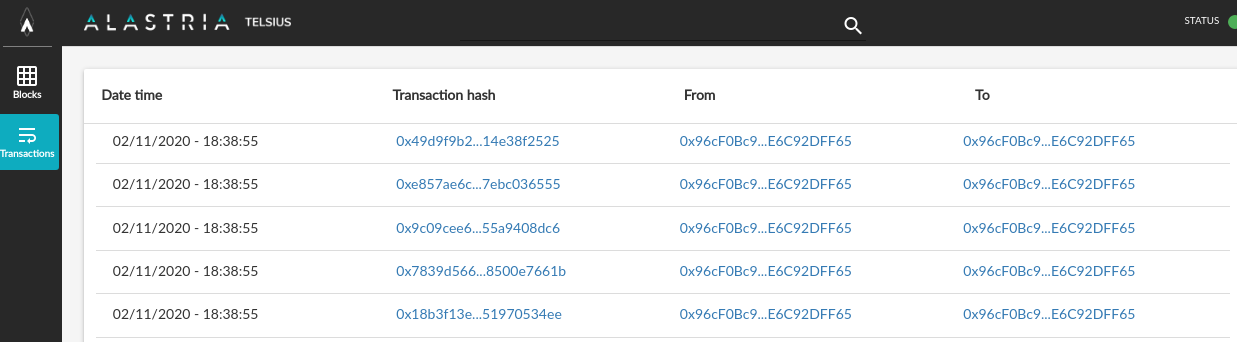
\includegraphics[width=1.0\textwidth]{Alastria-block-exporer.png}
                \caption{Alastria's Block explorer}
                \label{fig:alastria_block_explorer}
            \end{figure}
            \item \textbf{Immutability}. This property ensures that once something has been entered into the blockchain, it cannot be tampered or modified.
        \end{itemize}
        
        \subsubsection{How does Blockchain work?}
            A Blockchain is a growing list of records, called blocks, that are linked using cryptography. Each block contains a hash of the previous block, the timestamp and a batch of valid transaction hashes encoded into a Merkle tree. The linked blocks form a chain. This iterative process confirms the integrity of the previous block, all the way back to the original genesis block (the first block of the network).
            \begin{figure}[h]
                \centering
                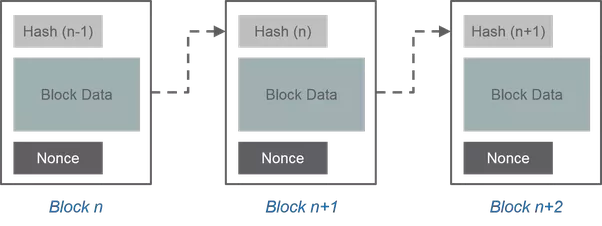
\includegraphics[width=1.0\textwidth]{block-example.png}
                \caption{Visual example of linked blocks}
                \label{fig:linked_blocks}
            \end{figure}
            
        \subsubsection{Types of blockchains}
            There are different kinds of Blockchain networks, each one with different features. One of the most common classification is according to the architecture. The following figure shows a table with the classification.
            \begin{figure}[h]
                \centering
                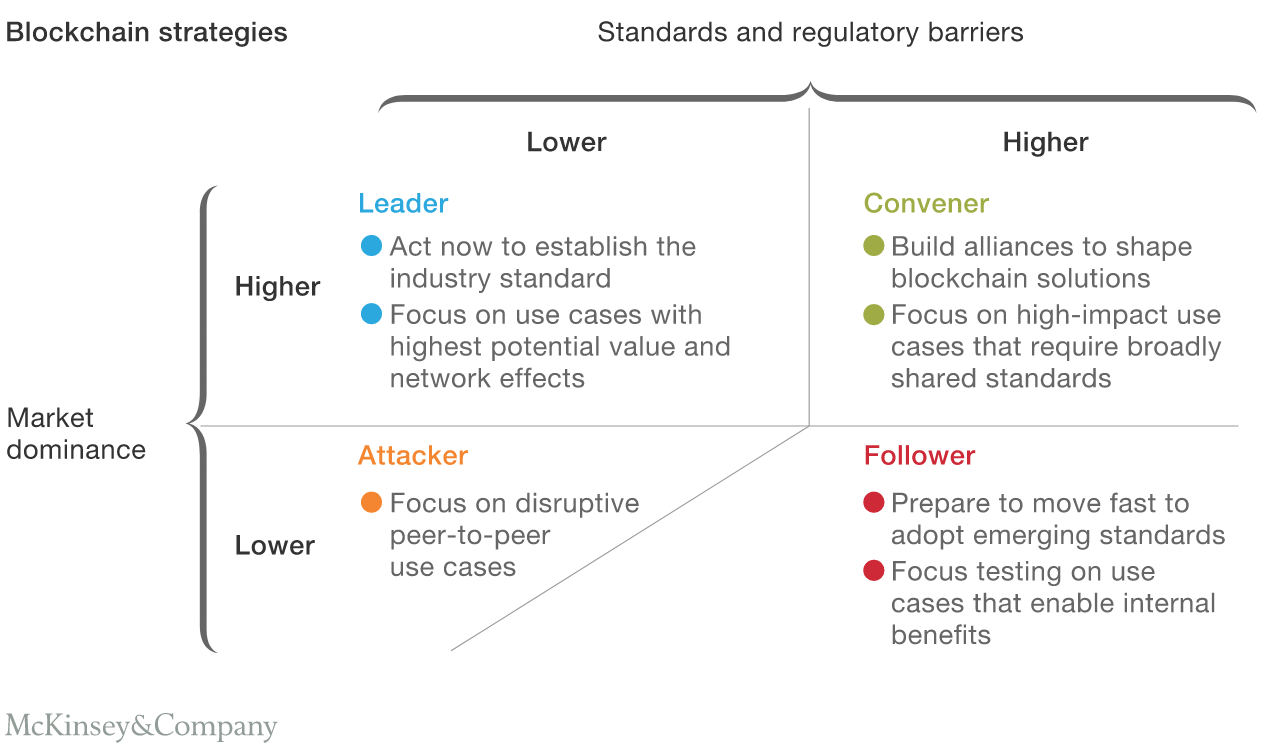
\includegraphics[width=1.0\textwidth]{Blockchain-types.png}
                \caption{Blockchain architecture classification by \textit{McKinsey\&Company}}
                \label{fig:blockchain_classification}
            \end{figure}

            \begin{itemize}
                \item \textbf{Public}. A public network is the one where everyone can join. Some examples of public networks are Bitcoin, Ethereum and Litecoin.
                \item \textbf{Private}. A private network is the one where only authorized members can join. Some examples of private networks are Quorum and Monax.
                \item \textbf{Permissionless}. A permissionless network is a private or public blockchain where every member can read and write.
                \item \textbf{Permissioned}. A permissioned network is a private or public blockchain where every member can read but only some can write. Some examples of public permissioned networks are Alastria and LACChain.
            \end{itemize}          
            Also, there are two more types of blockchain networks on the rise.
            \begin{itemize}
                \item \textbf{Consortium} or \textbf{hybrid networks}. These networks are private and permissioned, operated by known entities such as stakeholders of a given industry regrouped in a consortium or exploiting a shared platform. Some known examples are \textit{Hyperledger} \textit{Fabric}, \textit{R3 Corda} and \textit{Multichain}.
                \item \textbf{Blockchain as a Service} (BaaS). These are cloud platforms hosted by a service provider to deploy blockchain applications. The service provider manages the blockchain network while the customer defines the business logic. Some of the examples are \textit{Amazon (AWS)} and \textit{Oracle} blockchain platforms.
            \end{itemize}
            
            \subsubsection{Uses of blockchain}
                With the different properties of blockchain technology, and the different types of networks, there are a lot of use cases. The best known use case is using the blockchain as a payment infrastructure, the best example is Bitcoin. But there are a lot of other use cases shown in the next figure.\\
                \begin{figure}[h]
                    \centering
                    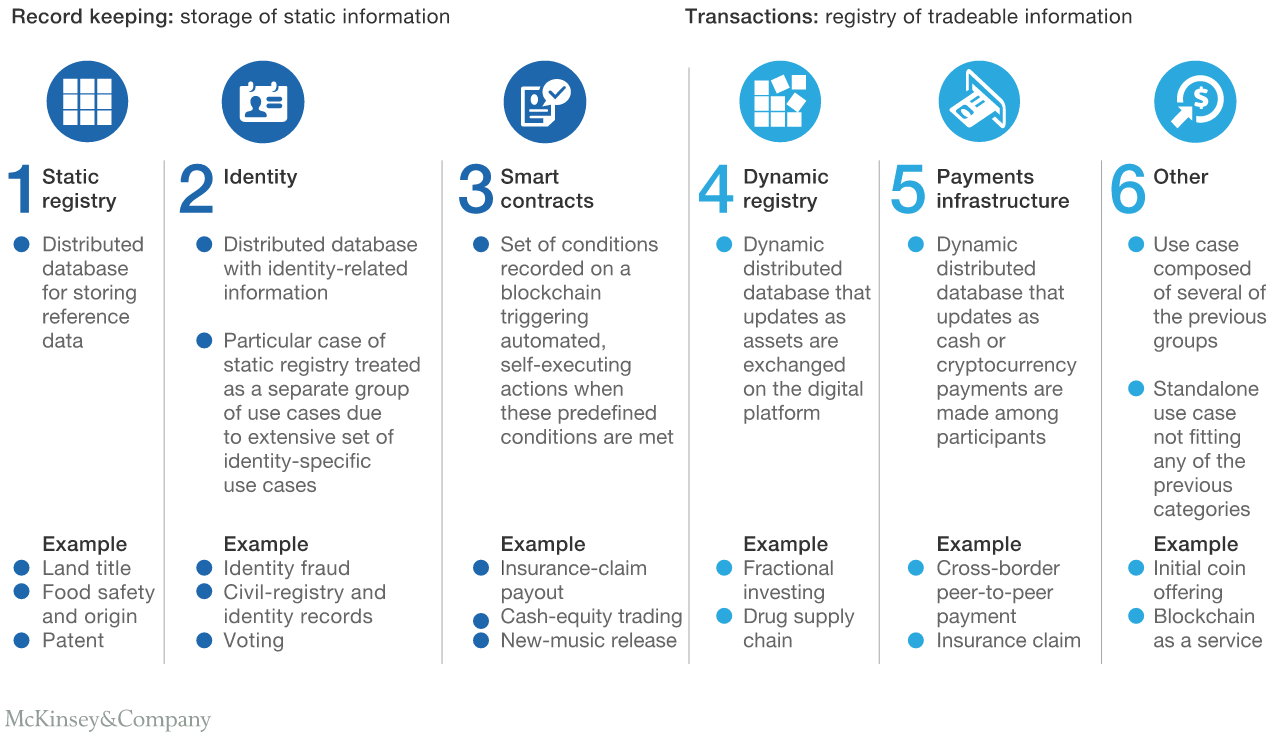
\includegraphics[width=0.95\textwidth]{Blockchain-uses.png}
                    \caption{Use cases table by \textit{McKinsey\&Company}}
                    \label{fig:blockchain_uses}
                \end{figure}
                
                In this document we are going to focus on the Self Sovereign Identity (SSI) using blockchain.

    \subsection{Ethereum}
        Ethereum is an open-source, public, blockchain-based distributed ledger featuring smart contract functionality. It enables developers to build blockchain applications with business logic that execute in a trustless environment, while leveraging the high availability of the Ethereum network. 
        \begin{figure}[h]
            \centering
            
\includegraphics[width=0.5\textwidth]{ethereum-logo-portrait-purple.png}
            \caption{Ethereum logo}
            \label{fig:ethereum_logo}
        \end{figure}
        The principles behind Ethereum philosophy are:
        \begin{itemize}
            \item \textbf{Simplicity}. The Ethereum protocol should be as simple as possible.
            \item \textbf{Universality}. Ethereum provides an internal Turing-complete scripting language. This language can be used to construct any logic, and any business case.
            \item \textbf{Modularity}. The Ethereum protocol is designed to be as modular as possible, to allow if one was to make a small protocol modification in one place, the application stack would continue to function as normally. 
            \item \textbf{Agility}. The protocol can be modified.
            \item \textbf{Non-discrimination} and \textbf{non-censorship}. The protocol should not restrict any usage.
        \end{itemize}
        
        \subsubsection{Ether}
            Ether (ETH) is the native cryptocurrency used on the Ethereum network and is used to compensate miners who secure transactions. It is used to pay for gas, a unit of computation used in transactions and other state transitions.
            Ether also has many current use cases, such as a store of value, a medium of exchange, and a unit of account.
            
        \subsubsection{Ethereum Accounts}
            An Ethereum account or simply an “account” is the combination of an Ethereum address and it’s private key. An account can hold balance (Ether) and can send transactions. In Ethereum there are 2 types of accounts.
            \begin{itemize}
                \item \textbf{Externally owned accounts} (EOA). These accounts are a combination of public address and private key. This accounts:
                \begin{itemize}
                    \item Has an ether balance
                    \item Can send transactions to Smart Contracts
                    \item Can send and receive ether to/from another account
                    \item Is controlled by private keys
                    \item Has no associated code
                \end{itemize}
                \item \textbf{Contract accounts}: These accounts don’t have a corresponding private key. These accounts are generated when a Smart Contract is deployed in the blockchain. They are normally called “contracts” instead of contract accounts. A contract:
                \begin{itemize}
                    \item Has an ether balance
                    \item They can receive ether just like EOA
                    \item Has associated code
                    \item Code execution is triggered by transactions or calls received from other contracts or accounts
                    \item When executed can manipulate its own persistent storage
                \end{itemize}
            \end{itemize}
        
        \subsubsection{Ethereum wallet}
            Wallets are software that are used to store and manage Ethereum accounts. Wallets allow the user to manage multiple accounts, provide functionality to sign transactions, track balances and so on. Wallets can be classified into two types.
            \begin{itemize}
                \item \textbf{Non-deterministic} wallet. These wallets use a random private key and generate a private key from it.
                \item \textbf{Deterministic} wallet. In this wallet, keys are derived from a seed. The seed allows a user to easily back up and restore a wallet without needing any other information, and in some cases allow the creation of public addresses without the knowledge of the private key.
            \end{itemize}
        
        \subsubsection{Ethereum stack}
            Like any software stack, the complete "Ethereum stack" will vary from project to project depending on your business goals. However, the typical layers are:
            \paragraph{Ethereum Virtual Machine (EVM)}
                The Ethereum Virtual Machine, normally known as EVM is a software designed to emulate a machine with certain capabilities that make the Ethereum blockchain possible. We can program instructions for the EVM, using a series of opcodes, which we can then compile and translate into a specific bytecode or language that the EVM can understand and execute.\\
                
                The opcodes perform standard stack operations like \textit{XORAND}, \textit{ADD}, \textit{SUB}, etc. The EVM also implements a number of blockchain-specific stack operations, such as \textit{ADDRESS}, \textit{BALANCE}, \textit{SHA3}, \textit{BLOCKHASH}, etc. More specific information can be found at \url{ https://www.ethervm.io/#opcodes}.\\
                
                To make programming easier for the virtual machine, a specialized high-level language called Solidity was created. This programming language is used to create Smart Contracts. Solidity first transforms opcodes and then these to bytecode. This bytecode is finally executed by the EVM to perform the specified operations of a  Smart Contract. All this means that the EVM can function as a real computer, executing from the simplest to the most complex operations.\\
                
                In the following sections we will talk in detail about the Smart Contracts and Solidity.
                
            \paragraph{EVM Characteristics}
                The EVM has a series of unique characteristics:
                \begin{itemize}
                    \item It provides a \textbf{high level of security}. As it is a virtual machine limited in the instructions (opcodes) and the way they are executed, EVM is capable of executing unreliable codes without disastrous consequences.
                    \item The EVM is a \textbf{completely decentralized} build. Each node within the Ethereum network runs a copy of the virtual machine and is synchronized with the rest of the nodes that make up the network. This guarantees that the instructions given by the EVM are executed as long as there is at least one active node. This allows access to the system from anywhere in the world, resisting censorship and guaranteeing access to network resources. Furthermore, it does not require the participation of third parties, and resources can’t be modified or altered.
                    \item Applications can be executed on the same blockchain network, without affecting other operations.
                    \item EVM is able to follow the “rules” of Smart Contracts.
                    \item The EVM has the ability to execute a series of well-defined opcodes.
                \end{itemize}
                
            \paragraph{How does it work?}
                The next figure defines how the EVM works.
                \begin{figure}[h]
                    \centering
                    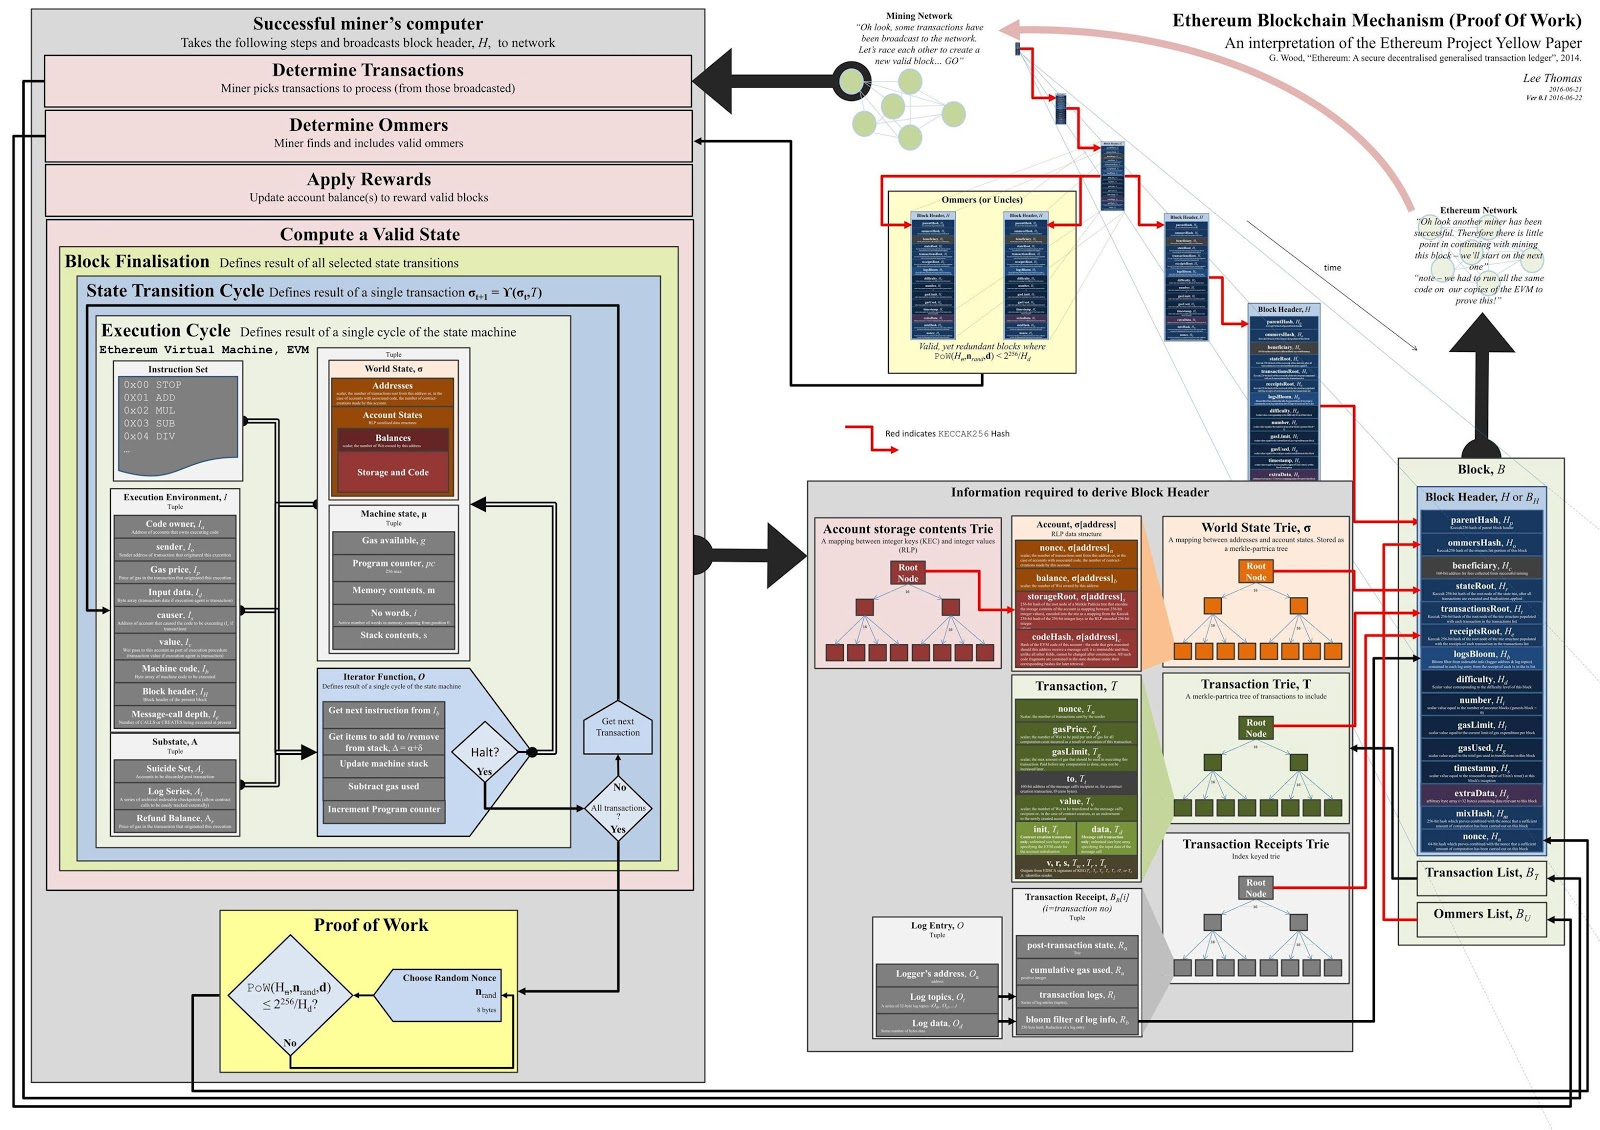
\includegraphics[width=1\textwidth]{evm-stack.jpeg}
                    \caption{EVM stack schema}
                    \label{fig:blockchain_stack}
                \end{figure}
                The Smart Contracts made with Solidity are compiled and converted to opcodes. These opcodes are transformed to bytecode, so it does facilitate the performance of the EVM tasks.\\

                Thus, each transaction and operation that is carried out on the Ethereum blockchain goes through this process, and its execution is carried out by the EVM, which at the end records everything on the Ethereum blockchain, leaving a public record of those operations. 

        \subsubsection{Smart Contracts}
            Sam Richards, a Software Engineer working on Ethereum defines the Smart Contract as 
            \begin{quote}
                \textit{“a snippet of code that runs on the Ethereum blockchain. It's a collection of functions and data that resides at a specific address on the Ethereum blockchain.}

                \textit{Smart contracts are a type of Ethereum account. This means they have a balance and they can send transactions over the network. However they're not controlled by a user, instead they are deployed to the network and run as programmed. User accounts can then interact with a smart contract by submitting transactions that execute a function defined on the smart contract. Smart contracts can define rules, like a regular contract, and automatically enforce them via the code.”}
            \end{quote}

        \subsubsection{Solidity}
            \begin{figure}[h]
                \centering
                
\includegraphics[width=0.4\textwidth]{solidity-logo.jpg}
                \caption{Solidity logo}
                \label{fig:solidity_logo}
            \end{figure}
            
            Solidity defines itself as an object-oriented, high-level language for implementing Smart Contracts. Smart Contracts are programs which govern the behaviour of accounts within the Ethereum state.\\
            
            Solidity was influenced by \textit{C++}, \textit{Python} and \textit{JavaScript} and is designed to target the Ethereum Virtual Machine (EVM). Solidity is statically typed, supports inheritance, libraries and complex user-defined types among other features.\\

            
            Below is a Smart Contract written in Solidity (Source code from \url{https://github.com/alastria/alastria-identity/blob/master/contracts/identityManager/AlastriaIdentityIssuer.sol}).
            \lstinputlisting[language=Solidity]{examples/SmartContracts/AlastriaIdentityIssuer.sol}
    
            More details about Solidity can be found in the official documentation. \url{https://solidity.readthedocs.io/en/latest/index.html}.
            
        \subsubsection{Ethereum Nodes}
            TODO
            
        \subsubsection{Ethereum Client APIs}
            TODO
            
        \subsubsection{End User Applications}
            TODO
            
        \subsubsection{Ethereum 2.0 (Eth2)}
            TODO

    \subsection{JSON-RPC}
                TODO
            
\section{Conclusions}

\nocite{*} % Cita todas las ref (incluidas las no citadas)
\printbibliography[heading=bibnumbered] % Última sección, numerada, para la bibliografía

\end{document}
